\chapter{Profiling Empirico para Particion Heterogenea CPU-GPU}

\section{4.1 Motivacion empirica y preguntas de medicion}
El profiling constituye la base empirica del resto del programa doctoral. Sin coeficientes de tiempo, energia, memoria y transferencia obtenidos de forma reproducible, cualquier formulacion de particion corre el riesgo de ser formalmente correcta pero operacionalmente fragil. Por ello, este capitulo no trata el profiling como una etapa auxiliar de benchmarking, sino como un mecanismo de inferencia experimental cuyo producto final son coeficientes robustos y auditables para optimizacion.

Las preguntas de medicion que guian el diseno son cinco. Primero, como medir costo por capa sin colapsar la heterogeneidad en promedios de modelo completo. Segundo, como separar en la medida de lo posible computo efectivo de overhead de despacho. Tercero, como representar transferencia inter-dispositivo de forma util para penalizar cortes de grafo. Cuarto, como robustificar las mediciones ante ruido y variabilidad inter-replica. Quinto, como preservar trazabilidad suficiente para que cada coeficiente pueda reconstruirse desde los artefactos fuente.

\section{4.2 Arquitectura de instrumentacion}
La arquitectura de instrumentacion se organiza alrededor del subsistema de profiling del proyecto y delega la captura operativa en el entrenador instrumentado y en componentes de soporte para politicas de precision, utilidades de sistema y extraccion estructural del grafo. El pipeline sigue una secuencia clara: parseo y normalizacion de entorno, evaluacion de politica de precision, carga de entradas preferentemente desde datasets reales, registro de hooks por modulo hoja, ejecucion de replicas y consolidacion de salidas tabulares y JSON. En terminos de implementacion, esta arquitectura se apoya en las capacidades de instrumentacion y ejecucion dinamica de PyTorch, pero las reordena hacia un contrato de evidencia mas estricto que el habitual en bibliotecas de entrenamiento generalista \cite{paszke2019pytorch}.

La instrumentacion por modulo hoja evita el doble conteo en estructuras anidadas y permite asociar a cada unidad de decision su costo observacional. Para cada capa se registran tiempos, energia, huellas de memoria y estimaciones de FLOPs; cuando existe soporte GPU, tambien se incorporan eventos y sincronizaciones necesarias para separar tiempo de pared observado y tiempo de kernel. Esta decision metodologica favorece una granularidad alineada con el problema de particion sin descender a un nivel de kernel primitivo que aumentaria ruido y complejidad semantica.

\section{4.3 Modelo de energia y carga computacional}
El proyecto aproxima la energia mediante potencia media observada por ventana temporal, lo que no constituye una medicion fisica perfecta por subsistema pero si una base comparativa consistente entre corridas. Esta aproximacion se combina con una heuristica de backward por capa y con formulas analiticas de FLOPs para los operadores dominantes, produciendo asi un conjunto de indicadores de costo utiles tanto para optimizacion como para interpretacion.

La inclusion simultanea de energia y carga computacional persigue un objetivo dual. Por un lado, amplifica la interpretabilidad del costo nodal mas alla de la mera latencia. Por otro, ayuda a distinguir capas aparentemente lentas por razones distintas: ineficiencia de kernel, saturacion de memoria o intensidad aritmetica insuficiente respecto al hardware local. En una tesis aplicada, esta contextualizacion es esencial para evitar conclusiones causales demasiado pobres.

\section{4.4 Politica de precision y validez}
Una fuente clasica de invalidez experimental en hardware heterogeneo es asumir que la precision solicitada coincide con la precision realmente ejecutada. En CPU modernas, ello depende de soporte ISA explicito; en GPU, de disponibilidad y comportamiento efectivo del backend. El pipeline resuelve este riesgo mediante sondeo de capacidades y metadatos de politica, registrando campos como \code{allowed}, \code{cpu_precision_executed}, \code{reason} y \code{status} para cada corrida o para cada omision justificada.

Esta compuerta de validez tiene tres efectos metodologicos. Primero, evita mezclar bajo una misma etiqueta mediciones obtenidas en regimens numericos distintos. Segundo, deja una huella auditable cuando una configuracion no puede ejecutarse. Tercero, reduce el riesgo de que los capitulos posteriores alimenten el ILP con coeficientes derivados de una precision nominal pero no efectiva.

\section{4.5 Extraccion estructural del grafo}
La extraccion estructural del grafo utiliza \code{torch.fx} como ruta principal y \code{torch.export} para ciertos modelos decoder-only que requieren una via alternativa. El objetivo no es producir un diagrama cosmetico del modelo, sino un conjunto de nodos y aristas con metadatos suficientes para enlazar nombres de capa, huellas de activacion y dependencias tensoriales. El campo \code{graph_trace_source} preserva la procedencia estructural de cada artefacto, lo cual permite distinguir evidencia metodologicamente admisible de rutas puramente diagnosticas. Esta exigencia de fidelidad estructural se alinea con la experiencia acumulada en trabajos de colocacion automatica y paralelizacion compilada, donde pequenas diferencias en la representacion del grafo alteran significativamente la calidad de la decision \cite{mirhoseini2017device,jia2019beyond,zheng2022alpa}.

Esta seccion tiene relevancia doctoral porque el costo de transferencia no puede formularse con rigor si la topologia se reduce a una cadena lineal artificial. Las conexiones residuales, los saltos y los patrones no secuenciales son precisamente los lugares donde una particion ingenua suele fallar. Por ello, el proyecto endurece la admisibilidad del grafo y relega el fallback lineal a un uso excepcional, no apto para sostener conclusiones principales.

\section{4.6 Modelo de transferencia consciente de arista}
El modelo de transferencia adoptado sigue una parametrizacion alpha-beta por direccion, distinguiendo host-a-dispositivo y dispositivo-a-host. Esta diferenciacion es necesaria porque las plataformas reales no suelen ofrecer simetria perfecta de ancho de banda y latencia, y una calibracion simetrica introduciria sesgo sistematico en el costo de corte. Sobre esta base se aplica una atenuacion conservadora por overlap, de modo que el costo efectivo no ignore la posibilidad de solapamiento entre computo y comunicacion, pero tampoco incurra en optimismo excesivo. Esta opcion metodologica dialoga con la literatura de pipeline y paralelizacion automatizada, donde el solapamiento parcial entre computo y transferencia es una fuente recurrente de divergencia entre costo ideal y costo materializado \cite{huang2019gpipe,narayanan2019pipedream,zheng2022alpa}.

El resultado final es un escalar de transferencia por arista consumible por el ILP. Su valor metodologico radica en traducir un fenomeno fisico del sistema en una magnitud optimizable, sin perder la posibilidad de auditar la procedencia de cada parametro. Este equilibrio entre realismo y tractabilidad es una de las piezas que distinguen al pipeline frente a un benchmarking tradicional por lotes completos.

\section{4.7 Agregacion estadistica robusta}
La agregacion de replicas se realiza sobre claves experimentales completas para evitar mezclar condiciones heterogeneas. Para cada canal numerico se calculan media, desviacion estandar y cuantiles superiores, y los coeficientes entregados al ILP se robustifican mediante el esquema $\hat{m}=\mu_m+k_\sigma\sigma_m$. Esta transformacion no es un detalle numerico menor, sino una declaracion metodologica explicita sobre el nivel de riesgo operacional que el experimento esta dispuesto a tolerar.

La presencia de \code{n_runs}, coeficientes de variacion y banderas de calidad convierte la agregacion en una compuerta inferencial. El sistema no solo resume mediciones; informa cuan confiable es el resumen. Esta decision es especialmente importante en resultados smoke, donde la dispersion puede ser alta y donde la tesis no debe confundir evidencia exploratoria con cierre estadistico definitivo.

\section{4.8 Validez experimental y reproducibilidad}
La validez interna del profiling se protege mediante replicas, control de semillas, politicas de preflight y exclusion explicita de corridas invalidas. La validez de construccion se fortalece al combinar tiempo, energia, memoria, transferencia e intensidad de computo, evitando que una unica metrica absorba por completo la semantica del problema. La validez externa, por su parte, se aborda mediante normalizacion por host y mediante la posibilidad de fusion multi-hardware de coeficientes, paso indispensable para cerrar la tesis con alcance transversal.

Como resultado del trabajo ya consolidado en \code{docs/CAPITULO_TESIS_PROFILING_ES.md}, este capitulo deja establecido que el profiling no es una fase preliminar prescindible. Es el fundamento empirico de la decision combinatoria posterior y, por tanto, una condicion necesaria para toda afirmacion sobre bondad de la particion.

Desde una perspectiva doctoral, este punto debe leerse con una cautela adicional. El profiling no es valioso solo porque mida, sino porque decide que cuenta como medida metodologicamente admisible. Una corrida aislada, desprovista de contexto numerico, precision efectiva o procedencia estructural, puede ser suficiente para depurar software; no lo es para sustentar una conclusion de tesis. El regimen inferencial del capitulo exige precisamente lo contrario: que cada coeficiente que alimenta el ILP sea el resultado de una secuencia de decisiones experimentales explicitadas y recuperables.

La Figura~\ref{fig:profiling-layer-costs} muestra un ejemplo real de esa instrumentacion sobre \code{simple_mlp}. En lugar de resumir el modelo completo en una unica latencia agregada, el artefacto separa costo forward en GPU, costo forward en CPU y penalizacion de transferencia consciente de arista para cada capa. Lo metodologicamente importante no es solo que existan diferencias absolutas entre capas, sino que el perfil resultante exhibe heterogeneidad interna suficiente para justificar una politica de asignacion selectiva en lugar de una colocacion monolitica.

\begin{figure}[t]
\centering
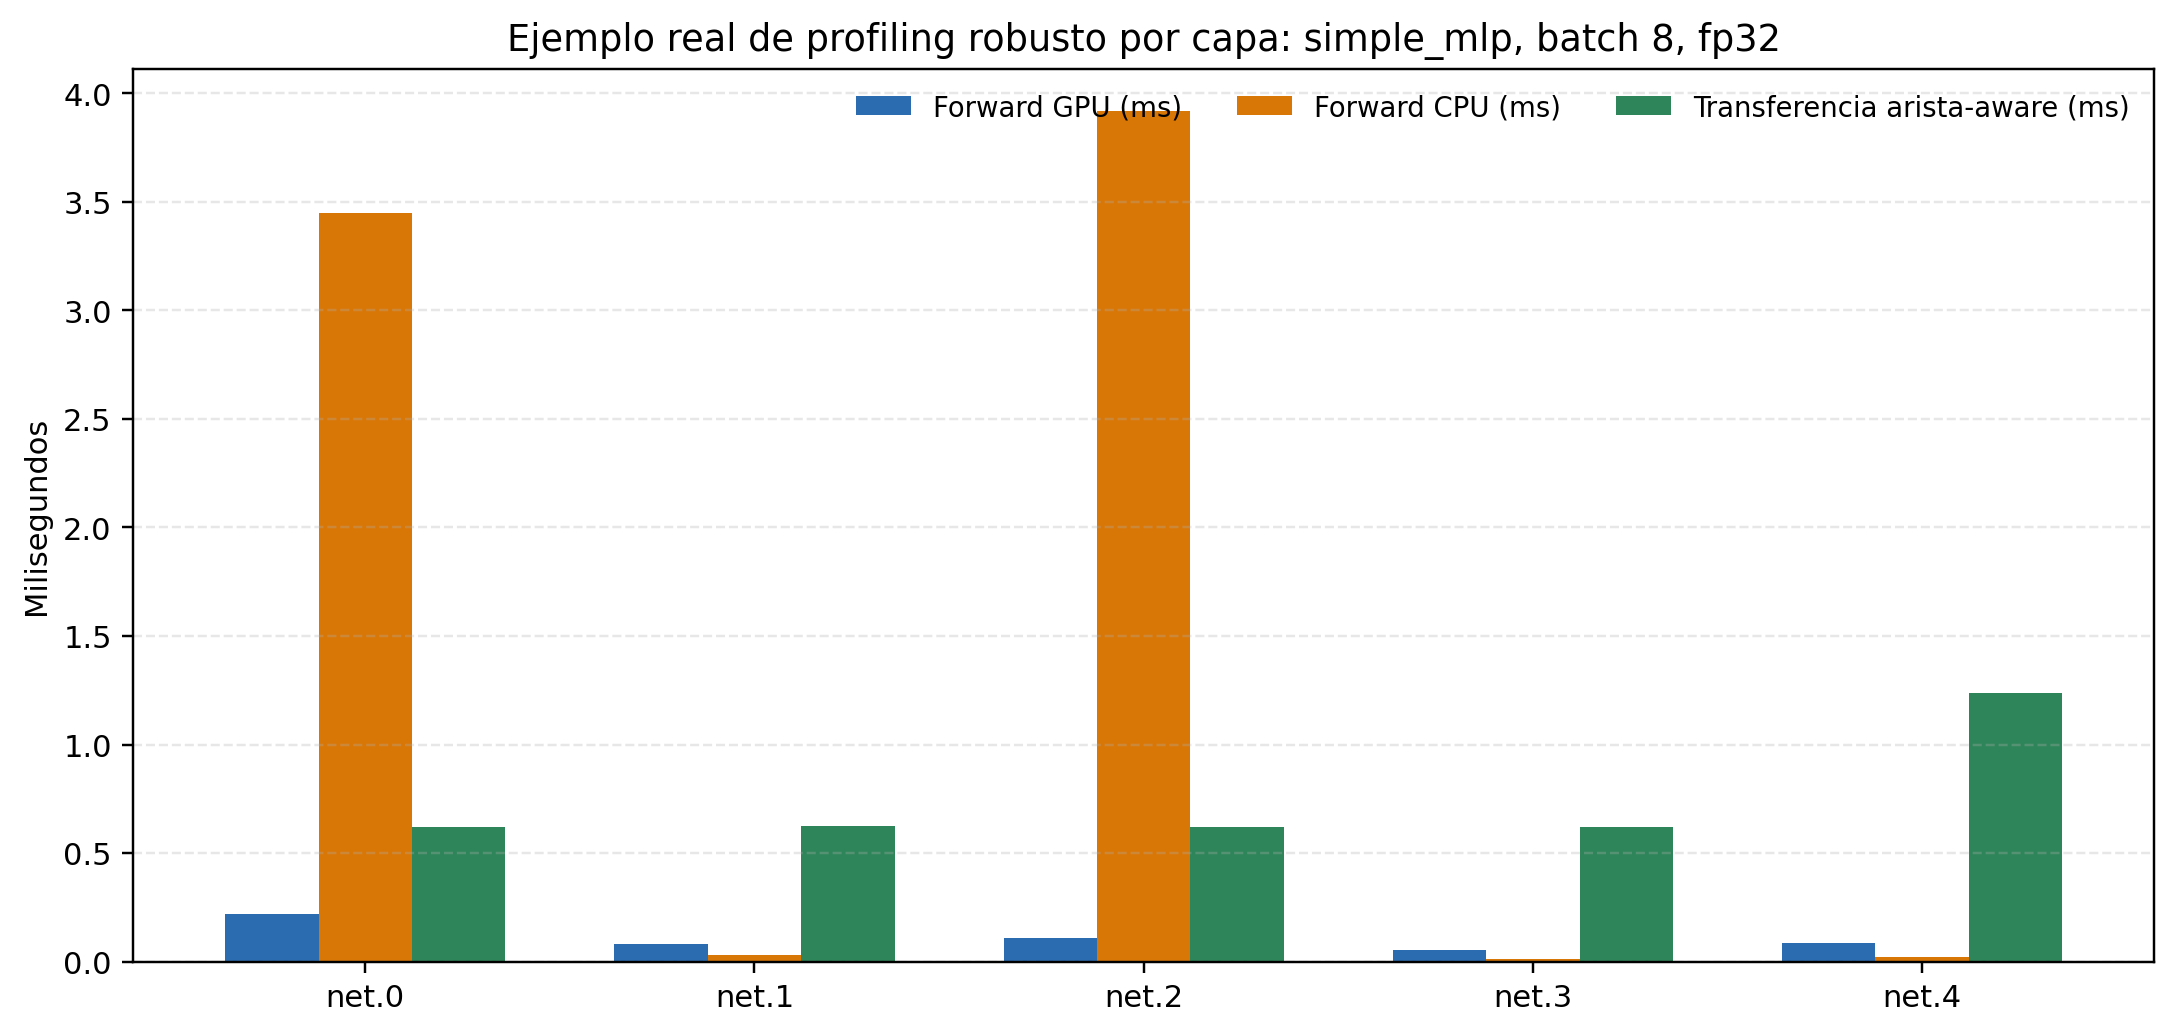
\includegraphics[width=0.95\textwidth]{../reports/thesis_figures/profiling_simple_mlp_layer_costs.png}
\caption{Perfil empirico real por capa para \code{simple_mlp} en smoke con batch 8 y precision \code{fp32}. La figura se genera directamente a partir de \code{simple_mlp_metrics_stats.csv}.}
\label{fig:profiling-layer-costs}
\end{figure}

\begin{table}[t]
\centering
\caption{Contrato minimo de artefactos del pipeline de profiling.}
\label{tab:profiling-artifacts}
\small
\begin{tabularx}{\textwidth}{l l X}
\toprule
Artefacto & Nivel & Rol metodologico \\
\midrule
\code{*_metrics.csv} & capa-corrida & Medicion cruda multicanal \\
\code{*_meta.json} & corrida & Contexto de hardware y politicas \\
\code{*_graph_nodes.csv} & estructura & Nodos con huellas de computo \\
\code{*_graph_edges.csv} & estructura & Dependencias y topologia util \\
\code{*_transfer_edges.csv} & arista & Costos calibrados de comunicacion \\
\code{*_metrics_stats.csv} & agregado & Coeficientes robustos para ILP \\
\bottomrule
\end{tabularx}
\normalsize
\end{table}

\begin{table}[t]
\centering
\caption{Extracto empirico de coeficientes robustos de profiling para \code{simple_mlp}.}
\label{tab:profiling-example-simple-mlp}
\scriptsize
\resizebox{0.92\textwidth}{!}{%
\begin{tabular}{lrrrrl}
\toprule
Capa & GPU fwd (ms) & CPU fwd (ms) & Transferencia (ms) & Memoria GPU (MB) & Calidad \\
\midrule
\code{net.0} & 0.220 & 3.448 & 0.622 & 19.335 & alta dispersion \\
\code{net.2} & 0.110 & 3.918 & 0.621 & 19.343 & alta dispersion \\
\code{net.4} & 0.088 & 0.022 & 1.235 & 19.343 & alta dispersion \\
\bottomrule
\end{tabular}
}
\normalsize
\end{table}

La Tabla~\ref{tab:profiling-example-simple-mlp} deja ver otra propiedad relevante: el problema no se reduce a escoger siempre GPU o siempre CPU. Las capas \code{net.0} y \code{net.2} muestran ventaja de tiempo en GPU pero con una penalizacion de transferencia comparable, mientras que \code{net.4} introduce una frontera de salida con costo comunicativo relativamente alto. Esta estructura de compromiso es precisamente la que vuelve razonable el paso desde profiling empirico hacia optimizacion declarativa.

\section{4.9 Del dato observado al coeficiente de decision}
Una contribucion metodologica menos visible, pero crucial, de este capitulo consiste en establecer la transformacion legitima entre observacion cruda y coeficiente de decision. El punto de partida no es una ecuacion cerrada, sino una nube de eventos con ruido, variabilidad de replica y dependencias contextuales. El punto de llegada no es una estadistica descriptiva neutra, sino un parametro que condiciona una decision binaria ejecutable. Entre ambos extremos media una cadena de validacion que incluye limpieza, agregacion, chequeo de dispersion, verificacion de precision y asociacion estructural con el grafo.

Este pasaje importa porque, en ausencia de dicha cadena, la optimizacion posterior quedaria epistemologicamente suspendida: seria imposible determinar si la solucion ILP mejora realmente la politica de asignacion o simplemente explota artefactos de medicion mal controlados. La tesis evita ese riesgo al convertir el profiling en una etapa con semantica inferencial propia. La decision combinatoria deja de apoyarse en numeros meramente disponibles y pasa a sostenerse en numeros metodologicamente justificados. La diferencia entre medicion disponible y coeficiente defendible es, de hecho, una de las lecciones que separa un benchmark utilitario de un pipeline de decision comparable con propuestas de colocacion automatica de mayor ambicion metodologica \cite{mirhoseini2017device,jia2019beyond}.

\begin{table}[t]
\centering
\caption{Cadena de transformacion desde observacion cruda hasta coeficiente util para optimizacion.}
\label{tab:profiling-inference-chain}
\small
\begin{tabularx}{\textwidth}{lX}
\toprule
Etapa & Funcion inferencial \\
\midrule
Medicion cruda por replica & Captura eventos, tiempos, energia y memoria bajo una configuracion concreta y versionable. \\
Control de validez & Verifica precision efectiva, soporte de hardware, semillas y consistencia basica de ejecucion. \\
Agregacion robusta & Resume tendencia central y dispersion sin colapsar la heterogeneidad experimental relevante. \\
Asociacion estructural & Vincula cada metrica con nodos y aristas del grafo computacional admisible. \\
Coeficiente para ILP & Entrega un escalar interpretable y trazable que puede entrar en funcion objetivo o restricciones. \\
\bottomrule
\end{tabularx}
\normalsize
\end{table}

\notaPendiente{Para la version de deposito conviene anadir aun dos figuras complementarias: la calibracion completa del modelo alpha-beta y una distribucion de replicas por canal para la campana multiservidor.}
